\subsection{\bf RQ3. Overlapping Analysis}

{\footnotesize{
\definecolor{mygray}{gray}{.9}
\begin{table}[t]
	\caption{RQ3. Overlapping Analysis. The number in the gray boxes: the unique bugs that the current approach can fix. P: \% of the bugs fixed by a tool and missed by the other.}
	\begin{center}
		\renewcommand{\arraystretch}{1}
		\begin{tabular}{p{1cm}<{\centering}|p{1.1cm}<{\centering}|p{0.8cm}<{\centering}|p{0.7cm}<{\centering}|p{1.1cm}<{\centering}|p{0.8cm}<{\centering}|p{0.7cm}<{\centering}}\hline
			Tool &\multicolumn{3}{c|}{Bugs.jar (1,158 Bugs)}&\multicolumn{3}{c}{BigFix (2,176 Bugs)}\\
			\hline
			{\bf CODIT}             & CODIT   & Overlap   & \tool  & CODIT   & Overlap   & {\tool} \\
			\hline
			Fixed \#     & \cellcolor{mygray} 6  & 80   & \cellcolor{mygray} 91  & \cellcolor{mygray} 13 &  157  & \cellcolor{mygray} 165 \\
			P            & 6.8\%   &    & 53.4\%  & 7.7\%   &    & 51.4\% \\
			\hline
			{\bf Tufano'19}             & Tufano 19'   & Overlap   & \tool  & Tufano 19'   & Overlap   & \tool \\
			\hline
			Fixed \#     & \cellcolor{mygray} 5  &  71  & \cellcolor{mygray} 101 & \cellcolor{mygray}4 & 85   & \cellcolor{mygray}237 \\
			P            &  6.2\%  &    &  58.8\% &  4.9\%  &    & 73.6\% \\
			\hline
			{\bf SequenceR}             & SequenceR   & Overlap   & \tool  & SequenceR   & Overlap   & \tool \\
			\hline
			Fixed \#     & \cellcolor{mygray} 7  &   95 & \cellcolor{mygray} 76 & \cellcolor{mygray} 23 &  158  & \cellcolor{mygray} 164 \\
			P            &   6.8\% &    & 44.6\%  &   11.2\% &    & 50.9\% \\
			\hline
			{\bf DLFix} & DLFix   & Overlap   & \tool  & DLFix   & Overlap   & \tool \\
			\hline
			Fixed \#     & \cellcolor{mygray}  19 &  105  & \cellcolor{mygray} 66 & \cellcolor{mygray}35 &  211  & \cellcolor{mygray}111 \\
			P            &  15.0\%  &    & 38.5\%  &  14.2\%  &    &  34.5\%\\
			\hline
			{\bf CoCoNuT}             & CoCoNuT   & Overlap   & \tool  & CoCoNuT   & Overlap   & \tool \\
			\hline
			Fixed \#     & \cellcolor{mygray} 20  & 120   & \cellcolor{mygray} 51 & \cellcolor{mygray}44 &  226  & \cellcolor{mygray} 96\\
			P            &  14.0\%  &    &  29.7\% &  16.1\%  &    & 29.7\% \\
			\hline
			{\bf CURE}             & CURE   & Overlap   & \tool  & CURE   & Overlap   & \tool \\
			\hline
			Fixed \#     & \cellcolor{mygray} 27  &  126  & \cellcolor{mygray} 45 & \cellcolor{mygray} 50&  233  & \cellcolor{mygray} 89\\
			P            &  17.4\%  &    & 26.4\%  & 17.7\%   &    &  27.7\%\\
			\hline
		\end{tabular}
		\label{RQ3_results}
	\end{center}
\end{table}
}}

To further study the comparison between {\tool} and the baseline
models, we peformed an overlapping analysis on the results.  In
Table~\ref{RQ3_results}, each row section corresponds to the
overlapping analysis between {\tool} and one baseline model
in two datasets.

\subsubsection{{\bf Comparison with CODIT}}

As seen in Table~\ref{RQ3_results}, in Bugs.jar, {\tool} can fix 91
bugs that CODIT missed and CODIT fixed 6 bugs that {\tool} missed,
while both can fix the same 80 bugs. Among the total number of bugs
fixed by both tools in Bugs.jar dataset, 53.4\% of them were fixed by
{\tool} and missed by CODIT, while only 6\% of them were fixed by
CODIT and missed by {\tool}. In BigFix dataset, while {\tool} can fix
165 bugs that CODIT missed, it missed only 13 bugs that CODIT can fix.

\begin{figure}[t]
	\centering
	\lstset{
		numbers=left,
		numberstyle= \tiny,
		keywordstyle= \color{blue!70},
		commentstyle= \color{red!50!green!50!blue!50},
		frame=shadowbox,
		rulesepcolor= \color{red!20!green!20!blue!20} ,
		xleftmargin=1.5em,xrightmargin=0em, aboveskip=1em,
		framexleftmargin=1.5em,
		numbersep= 5pt,
		language=Java,
		basicstyle=\scriptsize\ttfamily,
		numberstyle=\scriptsize\ttfamily,
		emphstyle=\bfseries,
		moredelim=**[is][\color{red}]{@}{@},
		escapeinside= {(*@}{@*)}
	}
	\begin{lstlisting}[]
public void visit(LOProject project) throws VisitorException {
    ...
(*@{\color{red}{-	\quad else if( op instanceof LOProject ) \{ }}@*)
(*@{\color{cyan}{+ \quad	else if( op instanceof ExpressionOperator ) \{}}@*)
		LogicalExpression expOper = exprOpsMap.get(op);
	...
	if (currentOp instanceof ExpressionOperator) {
		LogicalExpression exp = exprOpsMap.get(currentOp);
	...
}
	\end{lstlisting}
        \vspace{-15pt}
	\caption{Comparison with CODIT: An Example}
	\label{example_codit}
\end{figure}

Figure~\ref{example_codit} shows an example that were fixed by
{\tool}, but missed by CODIT. The correct fix is at line 4 by {\tool}:
\code{else} \code{if} \code{(op} \code{instanceof}
\code{ExpressionOperator)}.  However, CODIT fixed it into \code{else}
\code{if(} \code{op)}. This is an example that CODIT missed.
CODIT performs patch generation via translation of the buggy AST
sub-tree. It analyzes the buggy sub-tree that covers all the edited
nodes {\em without considering the surrounding context} in the method.
Thus, it did not fix this bug correctly. In this case, {\tool} could
leverage the surrounding code context at line 7 containing
\code{currentOp} \code{instanceof} \code{ExpressionOperator} to
generate the correct patch at line 4.

%{\color{blue}{1. CODIT only do the prediction and token generation on the buggy sub-tree that covers all edited nodes without considering the other information in the same method. So it cannot catch the information about the variable $ExpressionOperator$ in the method.
%2. Fixing results: \textit{CODIT: else if( op )$ \{$} CDFIX: \textit{else if( op instanceof ExpressionOperator ) $\{$}}}

\subsubsection{\bf Comparison with Tufano'19}

\begin{figure}[t]
	\centering
	\lstset{
		numbers=left,
		numberstyle= \tiny,
		keywordstyle= \color{blue!70},
		commentstyle= \color{red!50!green!50!blue!50},
		frame=shadowbox,
		rulesepcolor= \color{red!20!green!20!blue!20} ,
		xleftmargin=1.5em,xrightmargin=0em, aboveskip=1em,
		framexleftmargin=1.5em,
		numbersep= 5pt,
		language=Java,
		basicstyle=\scriptsize\ttfamily,
		numberstyle=\scriptsize\ttfamily,
		emphstyle=\bfseries,
		moredelim=**[is][\color{red}]{@}{@},
		escapeinside= {(*@}{@*)}
	}
	\begin{lstlisting}[]
private Tuple readFromMemory() {
    if (mContents.size() == 0) return null;
    if (mMemoryPtr < mContents.size()) {
(*@{\color{red}{-\quad\quad\quad     return ((ArrayList<Tuple>)mContents).get(mMemoryPtr++);}}@*)
(*@{\color{cyan}{+\quad\quad\quad    return ((List<Tuple>)mContents).get(mMemoryPtr++);}}@*)
	} else {
        return null;
	}
}
	\end{lstlisting}
        \vspace{-15pt}
	\caption{Comparison with Tufano19': An Example}
	\label{example_tufano19}
\end{figure}

As seen in Table~\ref{RQ3_results}, in Bugs.jar, {\tool} can fix 101
bugs (58.8\%) that Tufano'19 missed and Tufano'19 fixed only 5 bugs
(6.2\%) that {\tool} missed, while both can fix the same 71 bugs.
%Among the total number of bugs fixed by both tools in Bugs.jar
%dataset, 53.4\% of them were fixed by {\tool} and missed by CODIT,
%while only 6\% of them were fixed by CODIT and missed by {\tool}.
In BigFix dataset, while {\tool} can fix 237 bugs that Tufano'19
missed, it missed only 4 bugs that Tufano'19 can fix.

Figure~\ref{example_tufano19} shows an example that were fixed by
{\tool}, but missed by Tufano'19. For Tufano'19, the model uses a
{\em machine translation approach on the entire buggy method}
\code{readFromMemory}.  Because the model did not distinguish the
buggy statement from the surrounding context in training, during
fixing, the noise from the irrelevant statements in the method could
cause it {\em predict an incorrect statement to be fixed}. In this
example, Tufano'19 incorrectly identified line 2 as a buggy statement,
and fixed it into \code{if(} \code{mMemoryPtr.size} \code{()}
\code{==} \code{0)} \code{return} \code{null;}. The buggy line 4 was
correctly fixed into line 5 by {\tool}. By distinguishing the context
from the fixing changes, {\tool} could learn the type \code{List} of
\code{mContents} from lines 2 and 3 in which the method \code{size()} is
called on \code{mContents}.

%{\color{blue}{1. Tufano 19' learns and makes prediction only on the method level. In this case, it may fix the wrong position.
%2. Fixing results:
%Tufano 19': \textit{if (mMemoryPtr.size() == 0) return null;} (this fix at line 2)
%CDFIX: \textit{return ((List<Tuple>)mContents).get(mMemoryPtr++);}}}


%=============================================================

\subsubsection{\bf Comparison with SequenceR}

As seen in Table~\ref{RQ3_results}, in Bugs.jar dataset, {\tool} can
fix 76 bugs (44.6\%) that SequenceR missed and SequenceR fixed only 7
bugs (6.8\%) that {\tool} missed, while both can fix the same 95 bugs.
%Among the total number of bugs fixed by both tools in Bugs.jar
%dataset, 53.4\% of them were fixed by {\tool} and missed by CODIT,
%while only 6\% of them were fixed by CODIT and missed by {\tool}.
In BigFix dataset, among the total number of bugs fixed by either
tools, while {\tool} can fix 50.9\% (164 bugs) that SequenceR missed,
it missed only 11.2\% (23 bugs) that SequenceR can fix.

Figure~\ref{example_3} shows an example that SequenceR missed, but was
fixed correctly by {\tool}. Despite considering the context, {\em
  SequenceR treats source code as a sequence of code tokens}. However,
the fix from line 6 into line 7 involves structural changes to the AST
of the statement at line 6 because the order of two operations
\code{abs} and \code{\%} is changed.  In the buggy code, \code{abs} is
operated first and then \code{\%} is next. In the correct code,
\code{\%} is operated before \code{abs}. As shown in
Figure~\ref{tree-change}, the structure of the AST for the statement
is changed to reflect the change in that order. However, SequenceR
considers the statement as the sequence of tokens, and it just fixes
it by replacing the token \code{hashCode} with the token
\code{get}. That is, SequenceR incorrectly fixed the line 6 into
\code{return} \code{(Math.} \code{abs(} \code{keyTuple.} \code{get()}
\code{\%} \code{totalReducers);}.

%SequenceR: \textit{return (Math.abs( keyTuple.get()) \% totalReducers);}

\begin{figure}[t]
	\centering
	\lstset{
		numbers=left,
		numberstyle= \tiny,
		keywordstyle= \color{blue!70},
		commentstyle= \color{red!50!green!50!blue!50},
		frame=shadowbox,
		rulesepcolor= \color{red!20!green!20!blue!20} ,
		xleftmargin=1.5em,xrightmargin=0em, aboveskip=1em,
		framexleftmargin=1.5em,
		numbersep= 5pt,
		language=Java,
		basicstyle=\scriptsize\ttfamily,
		numberstyle=\scriptsize\ttfamily,
		emphstyle=\bfseries,
		moredelim=**[is][\color{red}]{@}{@},
		escapeinside= {(*@}{@*)}
	}
	\begin{lstlisting}[]
public int getPartition(PigNullableWritable wrappedKey, Writable value, int numPartitions) {
	....
	indexes = reducerMap.get(keyTuple);
	// if the reducerMap does not contain the key, do the default hash based partitioning
	if (indexes == null) {
(*@{\color{red}{-\quad\quad\quad  return (Math.abs(keyTuple.hashCode()) \% totalReducers);	}}@*)
(*@{\color{cyan}{+\quad\quad\quad     return (Math.abs(keyTuple.hashCode() \% totalReducers));}}@*)
	}
	....
}
	\end{lstlisting}
        \vspace{-12pt}
	\caption{Comparison with the context-aware APR baseline models: SequenceR, CoCoNuT, DLFix, and CURE}
	\label{example_3}
\end{figure}


\begin{figure}[t]
	\centering
	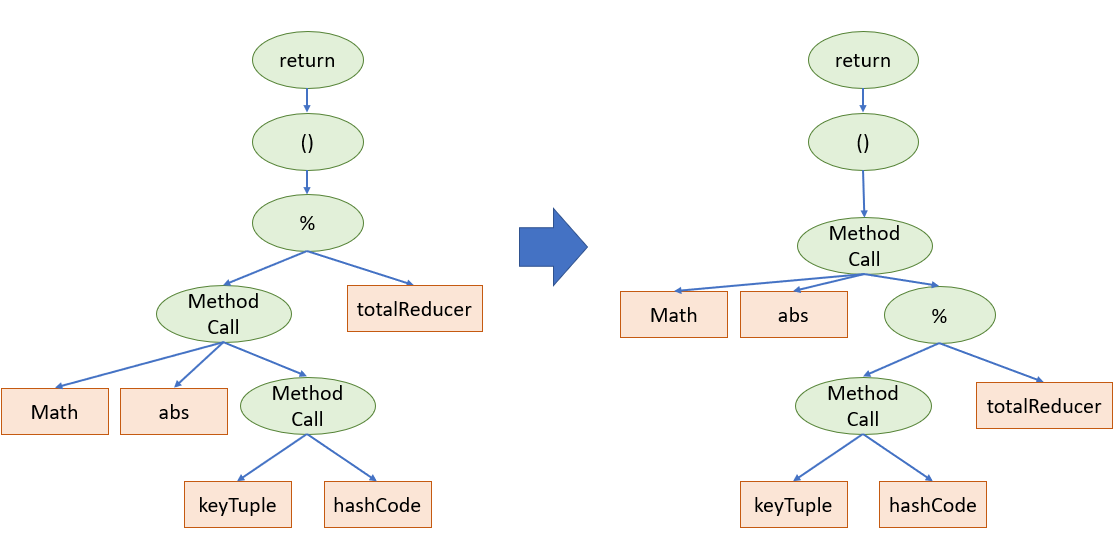
\includegraphics[width=3in]{graphs/example_3.png}
        \vspace{-6pt}
	\caption{AST Structure Changes for Fixing in Figure~\ref{example_3}}
	\label{tree-change}
\end{figure}


\subsubsection{\bf Comparison with CoCoNuT}

As seen in Table~\ref{RQ3_results}, in Bugs.jar, {\tool} can fix 51
bugs that CoCoNuT missed and CoCoNuT fixed 20 bugs that {\tool}
missed, while both can fix the same 120 bugs. Among the total
number of bugs fixed by both tools in BigFix dataset, 29.7\% of them
were fixed by {\tool} and missed by CoCoNuT, while only 16.1\% of them
were fixed by CoCoNuT and missed by {\tool}.

CoCoNuT did not fix correctly the example in Figure~\ref{example_3}.
It fixed line 6 into \code{return (} \code{Math.} \code{abs(}
\code{keyTuple.} \code{hashCode());}. First, CoCoNuT represents the
source code by a sequence of tokens, which is not well-suited for this
structural change in this example. Second, despite considering the
context, CoCoNuT encode the surrounding code as a feature in a single
model for learning the fix. {\tool} dedicates the context learning as
a model separately from the model for code transformation learning.
In this example, {\tool} is able to learn the structural change in the
AST (Figure~\ref{tree-change}).

\subsubsection{\bf Comparison with CURE}

As seen in Table~\ref{RQ3_results}, in Bugs.jar, {\tool} can fix 45
bugs that CURE missed and CURE fixed 27 bugs that {\tool} missed,
while both can fix the same 126 bugs. In BigFix dataset, the number of
unique bugs that were fixed by {\tool} but missed by CURE is almost
double the one that were fixed by CURE but missed by {\tool} (89
versus 50).

CURE did not fix correctly the example in Figure~\ref{example_3}. It
fixed the line 6 into \code{return (} \code{Math.} \code{abs(}
\code{keyTuple.} \code{hashCode())} \code{/} \code{totalReducers);}.
That is, it just replaced the operator \code{\%} with \code{/}.
Compared to CoCoNuT, CURE also represents source code as a sequence of
tokens, thus, is not well-suited to learn the structural changes for
the fix in this example. CURE is code-aware, however, similar to
CoCoNuT, it still encodes the code-aware features from the context
into a single model. {\tool} treats context learning with the CCL
model separately from transformation learning with the CTL model.

\subsubsection{\bf Comparison with DLFix}

As seen in Table~\ref{RQ3_results}, in Bugs.jar, {\tool} can fix 66
bugs that DLFix missed and DLFix fixed 19 bugs that {\tool}
missed, while both can fix the same 105 bugs. Among the total
number of bugs fixed by both tools in BigFix dataset, 34.5\% of them
were fixed by {\tool} and missed by DLFix, while only 14.2\% of them
were fixed by DLFix and missed by {\tool}.

DLFix also did not fix correctly the buggy code in
Figure~\ref{example_3}. It fixed the line 6 into \code{return (}
\code{Math.} \code{abs(} \code{keyTuple.} \code{hashCode())} \code{\%}
\code{curIndex);}. Despite that DLFix learns tree-structured code
transformations with separate models for context learning and
transformation learning, it follows a cascading architecture between
two models for such learning. Thus, the incorrect learning of context
might affect the learning of transformations. In {\tool}, context
learning and transformation learning are treated as a dual task
to propagate the impact on each other to help improve APR.


%{\color{blue}{1. SequenceR, CoCoNut, CURE all using sequence structure to do the code fixing. However, it is hard for them to learn the structure changes in this example. DLFix learns the structure changes, but it does not learn it as well as CDFix.
%2. Fixing results:
%SequenceR: \textit{return (Math.abs( keyTuple.get()) \% totalReducers);}
%CoCoNut: \textit{return (Math.abs( keyTuple.hashCode()));}

%DLFix: \textit{return (Math.abs( keyTuple.hashCode()) \% curIndex);}

%CURE: \textit{return (Math.abs( keyTuple.hashCode()) / totalReducers);}

%CDFIX: \textit{return (Math.abs( keyTuple.hashCode() \% totalReducers));}}}





%Table~\ref{RQ3_results} shows the overlapping analysis of the bugs fixed by {\tool} and the studied baselines. The results show that {\tool} can fix more unique bugs than any compared baseline. For example, {\tool} can fix 89 bugs that cannot be fixed by CURE, while CURE can fix 50 bugs that our {\tool} cannot fix.


%Consolidating results from RQ2 and RQ3, overall, {\tool} can auto-fix more bugs and unique bugs than any studied baselines, indicating that {\tool} is better and complementary to other baselines.
